 
\chapter{Quantile Regression}\label{chapter::quantile-regression}
 

\section{From the mean to the quantile}

For a random variable $y$, we can define its mean as 
\[
E(y)=\arg\min_{\mu  \in \mathbb{R} }E\left\{ (y-\mu)^{2}\right\} .
\]
With IID data $(y_{i})_{i=1}^{n}$, we can compute the sample mean
\[
\bar{y}=n^{-1}\sumn y_{i} = \arg\min_{\mu \in \mathbb{R} } n^{-1} \sumn (y_i-\mu)^{2} ,
\]
which satisfies the CLT: 
\[
\sqrt{n}(\bar{y}-E(y))\rightarrow\N(0, \var(y))
\]
in distribution if the variance $ \var(y)$ is finite. 


\begin{figure}[ht]
\centering
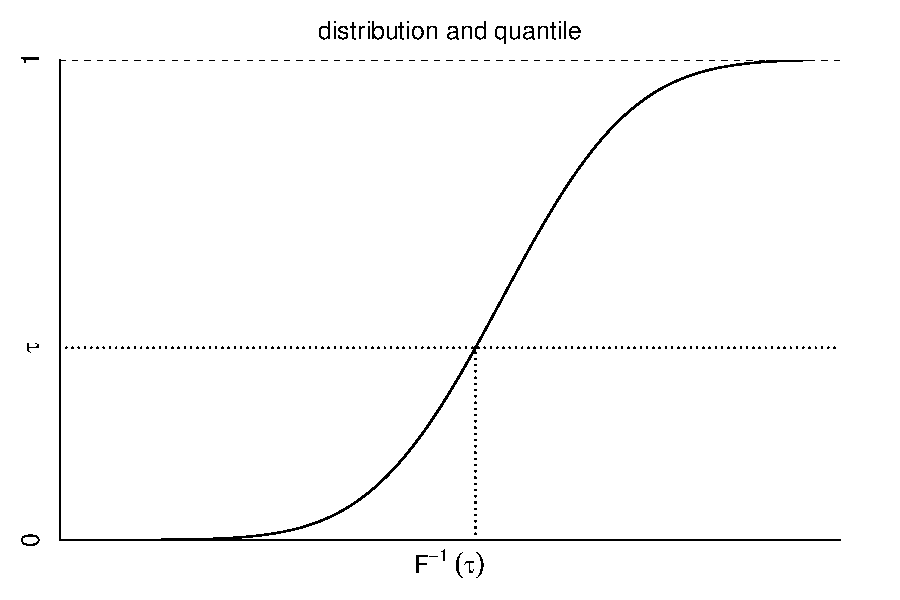
\includegraphics[width=0.8\textwidth]{figures/CDFquantile.pdf}
\caption{CDF and quantile}\label{fig::cdf-quantile}
\end{figure}


However, the mean can miss important information about $y$. How about other features of the outcome $y$? Quantiles can
characterize the distribution of $y$. For a random variable $y$,
we can define its distribution function as $F(c)=\pr(y\leq c)$ and
its $\tau$th quantile as
\[
F^{-1}(\tau)=\inf\left\{ q:F(q)\geq\tau\right\} .
\]
This defines a quantile function $F^{-1}:[0,1]\rightarrow\mathbb{R}$.
If the distribution function is strictly monotone, then the quantile
function reduces to the inverse of the distribution function, and the $\tau$-th quantile solves $\tau=\pr(y\leq q)$ as an equation of $q$.
See Figure \ref{fig::cdf-quantile}. For simplicity, this chapter focuses on the case with a  monotone distribution
function. The definition above formulates the mean as the minimizer of an objective function. Similarly, we can define quantiles in an equivalent
way below.
\begin{proposition}
\label{proposition:definitionofquantile}With a monotone distribution function
and positive density at the $\tau$th quantile, we have
\[
F^{-1}(\tau)=\arg\min_{q \in \mathbb{R} }E\left\{ \rho_{\tau}(y-q)\right\} ,
\]
where 
\[
\rho_{\tau}(u)=u\left\{ \tau-1(u<0)\right\} =\begin{cases}
u\tau, & \text{if }u\geq0,\\
-u(1-\tau), & \text{if }u<0,
\end{cases}
\]
is the check function (the name comes from its shape; see Figure \ref{fig::check-function}). In particular,
the median of $y$ is 
\[
\textup{median}(y)=F^{-1}(0.5)=\arg\min_{q \in \mathbb{R}}E\left\{ |y-q|\right\} .
\]
\end{proposition}
%
\begin{figure}
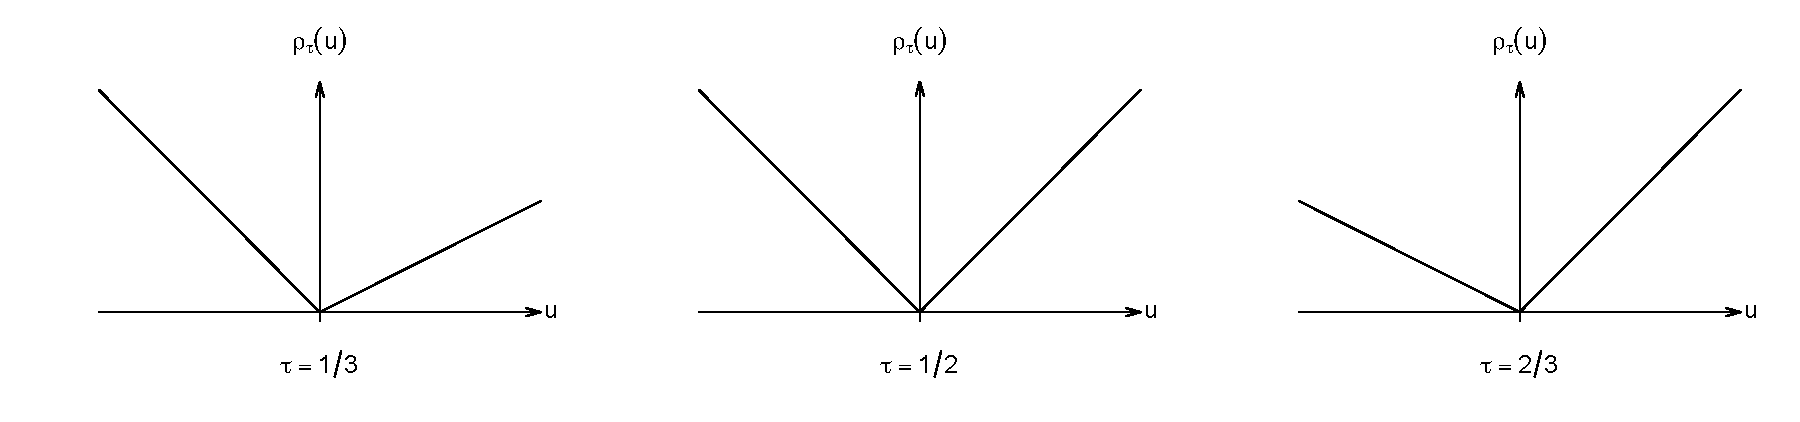
\includegraphics[width=\textwidth]{figures/checkfunctionplot}
\caption{Check function}\label{fig::check-function}
\end{figure}

\begin{myproof}{Proposition}{\ref{proposition:definitionofquantile}}
To simplify the proof, we further assume that $y$ has density function
$f(\cdot)$. We will use Leibniz's integral rule: 
\[
\frac{\d}{\d x}\left\{ \int_{a(x)}^{b(x)}f(x,t)\d t\right\} =f(x,b(x))b'(x)-f(x,a(x))a'(x)+\int_{a(x)}^{b(x)}\frac{\partial f(x,t)}{\partial x}\d t.
\]

We can write 
\[
E\left\{ \rho_{\tau}(y-q)\right\} =\int_{-\infty}^{q}(\tau-1)(c-q)f(c)\d c+\int_{q}^{\infty}\tau(c-q)f(c)\d c.
\]
To minimize it over $q$, we can solve the first-order condition
\[
\frac{\partial E\left\{ \rho_{\tau}(y-q)\right\} }{\partial q}=(1-\tau)\int_{-\infty}^{q}f(c)\d c-\tau\int_{q}^{\infty}f(c)\d c=0.
\]
So
\[
(1-\tau)\pr(y\leq q)-\tau\left\{ 1-\pr(y\leq q)\right\} =0
\]
which implies that
\[
\tau=\pr(y\leq q),
\]
so the $\tau$th quantile satisfies the first-order condition.
The second-order condition ensures it is the minimizer:
\[
\frac{\partial^{2}E\left\{ \rho_{\tau}(y-q)\right\} }{\partial q^{2}}\Big|_{q=F^{-1}(\tau)}=f\left\{ F^{-1}(\tau)\right\} >0
\]
by  Leibniz's integral rule again. 
\end{myproof}



The empirical distribution function is $\hat{F}(c)=n^{-1}\sumn1(y_{i}\leq c)$,
which is a step function, increasing but not strictly monotone. With
Proposition \ref{proposition:definitionofquantile}, we can easily define
the sample quantile as 
\[
\hat{F}^{-1}(\tau)=\arg\min_{q \in \mathbb{R}  }n^{-1}\sumn\rho_{\tau}(y_{i}-q),
\]
which may not be unique even though the population quantile is. We
can view $\hat{F}^{-1}(\tau)$ as a set containing all minimizers,
and with large samples the values in the set do not differ much. Similar
to the sample mean, the sample quantile also satisfies a CLT. 


\begin{theorem}\label{thm::sample-quantiles-asymptotics}
Assume $(y_{i})_{i=1}^{n}\iidsim y$ with distribution function $F(\cdot)$
that is strictly increasing and density function $f(\cdot)$ that
is positive at the $\tau$th quantile. The sample quantile
is consistent for the true quantile and is asymptotically Normal:
\[
\sqrt{n}\left\{ \hat{F}^{-1}(\tau)-F^{-1}(\tau)\right\} \rightarrow\N\left(0,\frac{\tau(1-\tau)}{\left[f\left\{ F^{-1}(\tau)\right\} \right]^{2}}\right)
\]
in distribution. In particular, the sample median satisfies
\[
\sqrt{n}\left\{ \hat{F}^{-1}(0.5)-\textup{median}(y)\right\} \rightarrow\N\left(0,\frac{1}{4\left[f\left\{ \textup{median}(y)\right\} \right]^{2}}\right)
\]
in distribution. 
\end{theorem}


\begin{myproof}{Theorem}{\ref{thm::sample-quantiles-asymptotics}}
Based on the first order condition in  Proposition \ref{proposition:definitionofquantile}, the population quantile solves
$$
E \{ m_\tau(y - q) \} =0,
$$
and the sample quantile solves
$$
n^{-1} \sumn m_\tau(y_i - q)  = 0,
$$
where the check function has a partial derivative with respect to
$u$ except for the point $0$: 
\begin{eqnarray*}
m_{\tau}(u) &=&  (\tau-1)1(u<0)+\tau1(u>0) \\
&=&\tau-1(u < 0).
\end{eqnarray*}
By Theorem \ref{theorem:sandwich-theorem-cov-iid},  we only need to find the bread and meat matrices, which are scalars now:
\begin{eqnarray*}
B &=& \frac{\partial   E \{ m_\tau(y - q) \}  }{ \partial q}\Big | _{q = F^{-1}(\tau)}\\
&=& \frac{\partial   E \{ \tau-1(y\leq q) \}  }{ \partial q}\Big | _{q =F^{-1}(\tau)}\\
&=& -\frac{\partial   F(q)   }{ \partial q}\Big | _{q =F^{-1}(\tau)}\\
&=& -f\{F^{-1}(\tau) \},
\end{eqnarray*}
and
\begin{eqnarray*}
M &=& E \left[ \{ m_\tau(y - q) \}^2 \right] \Big | _{q =F^{-1}(\tau)} \\
&=& E \left[ \left\{ \tau-1(y\leq q) \right\}^2 \right] \Big | _{q =F^{-1}(\tau)} \\
&=& E \left[ \tau^2 + 1(y\leq q) - 2\cdot  1(y\leq q) \tau \right] \Big | _{q =F^{-1}(\tau)} \\
&=& \tau^2 + \tau - 2\tau^2 \\
&=& \tau(1-\tau).
\end{eqnarray*}
Therefore, $\sqrt{n}\{ \hat{F}^{-1}(\tau)-F^{-1}(\tau)\}$ converges to Normal with mean zero and variance $M/B^2 = \tau(1-\tau)/ [f\{F^{-1}(\tau) \}]^2$. 
\end{myproof}



To conduct statistical inference for the quantile $F^{-1}(\tau)$, we need to estimate the density of $y$ at the $\tau$th quantile to obtain the estimated standard error of $\hat{F}^{-1}(\tau)$. Alternatively, we can use the bootstrap to obtain the estimated standard error. We will discuss the inference of quantiles in \ri{R} in Section \ref{section::numerical-examples-qr}. 



\section{From the conditional mean to conditional quantile}

With an explanatory variable $x$ for outcome $y$, we can define
the conditional mean as
\[
E(y\mid x)=\arg\min_{m(\cdot)}E\left[\left\{ y-m(x)\right\} ^{2}\right].
\]
We can use a linear function $x^{\T}\beta$ to approximate the conditional
mean with the population OLS coefficient 
\[
\beta=\arg\min_{b \in \mathbb{R}^p  }E\left\{ (y-x^{\T}b)^{2}\right\} =\left\{ E(xx^{\T})\right\} ^{-1}E(xy),
\]
and the sample OLS coefficient
\[
\hat{\beta}=\left(n^{-1}\sumn x_{i}x_{i}^{\T}\right)^{-1}\left(n^{-1}\sumn x_{i}y_{i}\right).
\]
We have discussed the statistical properties of $\hat{\beta}$ in previous chapters.
Motivated by Proposition \ref{proposition:definitionofquantile}, we can
define the conditional quantile function as 
\[
F^{-1}(\tau\mid x)=\arg\min_{q(\cdot)}E\left[\rho_{\tau}\left\{ y-q(x)\right\} \right].
\]
We can use a linear function $x^{\T}\beta(\tau)$ to approximate the
conditional quantile function with
\[
\beta(\tau)=\arg\min_{b   \in \mathbb{R}^p  }E\left\{ \rho_{\tau}(y-x^{\T}b)\right\} 
\]
called the $\tau$th population regression quantile, and 
\begin{equation}
\hat{\beta}(\tau)=\arg\min_{b   \in \mathbb{R}^p }n^{-1}\sumn\rho_{\tau}(y_{i}-x_{i}^{\T}b)\label{eq:sample-regression-quantiles}
\end{equation}
called the $\tau$th sample regression quantile. 
As a special case, when $\tau = 0.5$, we have the regression median:
\[
\hat{\beta}(0.5)=\arg\min_{b  \in \mathbb{R}^p  } n^{-1}\sumn |y_{i}-x_{i}^{\T}b|,
\]
which is also called the least absolute deviations (LAD).


\citet{koenker1978regression} started the literature under a correctly specified conditional quantile model:
$$
F^{-1}(\tau\mid x) = x^{\T} \beta(\tau).
$$
The interpretation of the $j$-th coordinate of the coefficient, $\beta_j(\tau)$, is the partial influence of $x_{ij}$ on the $\tau$th conditional quantile of $y_i$ given $x_{i}$. 
\citet{angrist2006quantile} discussed quantile regression under misspecification, viewing it as the best linear approximation to the true conditional quantile function. This chapter will focus on the statistical properties of
the sample regression quantiles following \citet{angrist2006quantile}'s discussion of statistical inference allowing for the misspecification of the quantile regression model. 
 
 
Before that, we first comment
on the population regression quantiles based on some generative models. Below assume that the $v_{i}$'s are IID independent of the covariates $x_i$'s, with mean zero and distribution $g(c) = \pr(  v_i \leq c)$. 



\begin{example}
Under the linear model $y_{i}=x_{i}^{\T}\beta+\sigma v_{i}$, we can verify that 
$$
E(y_i\mid x_i) = x_{i}^{\T}\beta
$$
and
\[
F^{-1}(\tau\mid x_{i})=x_{i}^{\T}\beta+\sigma g^{-1}(\tau).
\]
Therefore, with the first regressor being $1$, we have
\[
\beta_{1}(\tau)=\beta_{1}+\sigma g^{-1}(\tau),\quad\beta_{j}(\tau)=\beta_{j},\quad(j=2,\ldots,p).
\]
In this case, both the true conditional mean and quantile functions are linear, and
the population regression quantiles are constant across $\tau$ except
for the intercept.
\end{example}




\begin{example}
Under a heteroskedastic linear model $y_{i}=x_{i}^{\T}\beta+(x_{i}^{\T}\gamma)v_{i}$
with   $x_{i}^{\T}\gamma>0$ for all $x_{i}$'s,
we can verify that 
$$
E(y_i\mid x_i) = x_{i}^{\T}\beta
$$
and 
\[
F^{-1}(\tau\mid x_{i})=x_{i}^{\T}\beta+x_{i}^{\T}\gamma g^{-1}(\tau).
\]
Therefore, 
\[
\beta(\tau)=\beta+\gamma g^{-1}(\tau).
\]
In this case, both the true conditional quantile functions are linear, and
all coordinates of the population regression quantiles vary with $\tau$. 
\end{example}



\begin{example}
Under the transformed linear model $\log y_{i}=x_{i}^{\T}\beta+\sigma v_{i}$, we can verify that 
$$
E(y_i\mid x_i) = \exp(x_{i}^{\T}\beta) M_v(\sigma),
$$
where $M_v(t) = E(e^{tv})$ is the moment generating function of $v$, 
and 
\[
F^{-1}(\tau\mid x_{i})=\exp\left\{ x_{i}^{\T}\beta+\sigma g^{-1}(\tau)\right\} .
\]
In this case, both the true conditional mean and quantile functions are log-linear in covariates. 
\end{example}
   

\section{Sample regression quantiles}

\subsection{Computation}

The regression quantiles (\ref{eq:sample-regression-quantiles}) do
not have explicit formulas in general, and we need to solve the optimization
problem numerically. Motivated by the piece-wise linear feature of
the check function, we decompose $y_{i}-x_{i}^{\T}\beta$ into the
difference between its positive part and negative part:
\[
y_{i}-x_{i}^{\T}\beta=u_{i}-v_{i},
\]
where 
\[
u_{i}=\max(y_{i}-x_{i}^{\T}\beta,0),\quad v_{i}=-\min(y_{i}-x_{i}^{\T}\beta,0).
\]
So the objective function simplifies to the summation of 
\[
\rho_{\tau}(y_{i}-x_{i}^{\T}\beta)=\tau u_{i}+(1-\tau)v_{i},
\]
which is simply a linear function of the $u_{i}$'s and $v_{i}$'s.
Of course, these $u_{i}$'s and $v_{i}$'s are not arbitrary because
they must satisfy the constraints by the data. Using the notation
\[
Y=\left(\begin{array}{c}
y_{1}\\
\vdots\\
y_{n}
\end{array}\right),\quad X=\left(\begin{array}{c}
x_{1}^{\T}\\
\vdots\\
x_{n}^{\T}
\end{array}\right),\quad u=\left(\begin{array}{c}
u_{1}\\
\vdots\\
u_{n}
\end{array}\right),\quad v=\left(\begin{array}{c}
v_{1}\\
\vdots\\
v_{n}
\end{array}\right),
\]
finding the $\tau$th regression quantile is equivalent to a linear
programming problem with linear objective function and linear constraints:
\begin{align*}
 & \min_{b,u,v}  \tau1_{n}^{\T}u+(1-\tau)1_{n}^{\T}v  ,\\
 & \text{s.t. }Y=Xb+u-v,\\
 &\text{and } u_i \geq  0, v_i \geq  0 \quad  (i=1,\ldots, n).
\end{align*}
The function \ri{rq} in the \ri{R} package \ri{quantreg} computes the regression quantiles with various choices of methods. 

\subsection{Asymptotic inference}

Similar to the sample quantiles, the regression quantiles are also
consistent for the population regression quantiles and asymptotically
Normal. So we can conduct asymptotic inference based on the results
in the following theorem \citep{angrist2006quantile}.


\begin{theorem}\label{thm::regression-quantiles-asymptotics}
Assume $(y_{i},x_{i})_{i=1}^{n}\iidsim(y,x)$. Under some regularity
conditions, we have
\[
\sqrt{n}\left\{ \hat{\beta}(\tau)-\beta(\tau)\right\} \rightarrow\N(0,B^{-1}MB^{-1})
\]
in distribution, where 
\[
B=E\left[f_{y\mid x}\left\{ x^{\T}\beta(\tau)\right\} xx^{\T}\right],\quad M=E\left[\left\{ \tau-1\left(y-x^{\T}\beta(\tau)\leq0\right)\right\} ^{2}xx^{\T}\right],
\]
with $f_{y\mid x}(\cdot)$ denoting the conditional density of $y$
given $x$.
\end{theorem}


\begin{myproof}{Theorem}{\ref{thm::regression-quantiles-asymptotics}}
%Except for the point $0$,  the check function has a partial derivative with respect to
%$u$:
%\[
%m_{\tau}(u)=(\tau-1)1(u<0)+\tau1(u>0)=\tau-1(u\leq0).
%\]
The population regression quantile solves
\[
E\left\{ m_{\tau}(y-x^{\T}b)x\right\} =0,
\]
and the sample regression quantile solves
\[
n^{-1}\sumn m_{\tau}(y_{i}-x_{i}^{\T}b)x_{i}=0.
\]
By Theorem \ref{theorem:sandwich-theorem-cov-iid}, 
we only need to calculate the explicit forms of $B$
and $M$. Let $F_{y\mid x}(\cdot)$ and $f_{y\mid x}(\cdot)$ be the
conditional distribution and density functions. We have
\begin{align*}
E\left\{ m_{\tau}(y-x^{\T}b)x\right\}  & =E\left[\left\{ \tau-1(y-x^{\T}b\leq0)\right\} x\right]\\
 & =E\left[\left\{ \tau-F_{y\mid x}(x^{\T}b)\right\} x\right],
\end{align*}
so 
\[
\frac{\partial E\left\{ m_{\tau}(y-x^{\T}b)x\right\} }{\partial b^{\T}}
=-E\left\{ f_{y\mid x}(x^{\T}b)xx^{\T}\right\} .
\]
This implies the formula of $B$. The formula of $M$ follows from
\begin{align*}
M & =E\left\{ m_{\tau}^{2}(y-x^{\T}\beta(\tau))xx^{\T}\right\} \\
 & =E\left[\left\{ \tau-1(y-x^{\T}\beta(\tau)\leq0)\right\} ^{2}xx^{\T}\right].
\end{align*}
\end{myproof}



Based on Theorem \ref{thm::regression-quantiles-asymptotics}, we can estimate the asymptotic covariance matrix of $\hat{\beta}(\tau)$ by $n^{-1} \hat{B}^{-1} \hat{M}  \hat{B}^{-1}$, where
\[
\hat{M}=n^{-1}\sumn\left\{ \tau-1\left(y_{i}-x_{i}^{\T}\hat{\beta}(\tau)\leq0\right)\right\} ^{2}x_{i}x_{i}^{\T}
\]
and
\[
\hat{B}=\left(2nh\right)^{-1}\sumn1\left\{ |y_{i}-x_{i}^{\T}\hat{\beta}(\tau)|\leq h\right\} x_{i}x_{i}^{\T}
\]
for a carefully chosen $h$. \citet{powell1991estimation}'s theory suggests to use $h$ satisfying condition $h=O(n^{-1/3})$, but the theory is not so helpful since it only suggests the order of $h$. The \ri{quantreg} package in \ri{R} chooses a specific $h$ that satisfies this condition. 
In finite samples, the bootstrap often gives a better estimation of the asymptotic covariance matrix. 



\section{Numerical examples}\label{section::numerical-examples-qr}

\subsection{Sample quantiles}


\begin{figure}[ht]
\centering
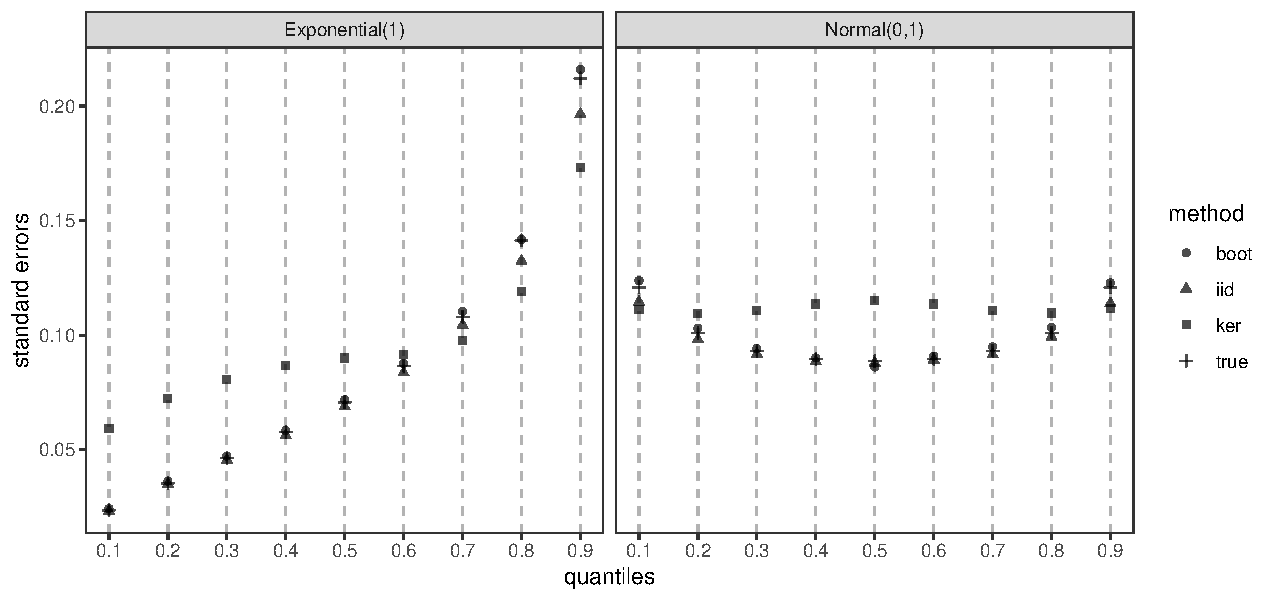
\includegraphics[width = \textwidth]{figures/ese_quantiles.pdf}
\caption{Standard errors for sample quantiles}\label{fig::se-sample-quantiles}
\end{figure}



We can use the \ri{quantile} function to obtain the sample quantiles. However, it does not report standard errors. Instead, we can use the \ri{rq} function to compute sample quantiles by regressing the outcome on constant 1. These two functions may return different sample quantiles when they are not unique. The difference is often small with large sample sizes. 


I use the following simulation to compare various methods for standard error estimation. The first data-generating process has a standard Normal outcome. 

\begin{lstlisting}
library(quantreg)
mc= 2000
n = 200
taus = (1:9)/10
get.se = function(x){x$coef[1,2]}
q.normal = replicate(mc,{
  y  = rnorm(n)
  qy = rq(y~1, tau = taus)
  se.iid = summary(qy, se = "iid")
  se.ker = summary(qy, se = "ker")
  se.boot= summary(qy, se = "boot")
  
  qy = qy$coef
  se.iid = sapply(se.iid, get.se)
  se.ker = sapply(se.ker, get.se)
  se.boot= sapply(se.boot, get.se)
  
  c(qy, se.iid, se.ker, se.boot)
})
\end{lstlisting}


In the above, \ri{se = "iid"}, \ri{se = "ker"}, and \ri{se = "boot"} correspond to the standard errors by \citet{koenker1978regression}, \citet{powell1991estimation}, and the bootstrap. 
I also run the same simulation but replace the Normal outcome with Exponential: \ri{y  = rexp(n)}. Figure \ref{fig::se-sample-quantiles} compares the estimated standard errors with the true asymptotic standard error in Theorem \ref{thm::sample-quantiles-asymptotics}. Bootstrap works the best, and the one involving kernel estimation of the density seems biased. 






\subsection{OLS versus LAD}


I will use simulation to compare OLS and LAD. In \ri{rq}, the default value is \ri{tau=0.5}, fitting the LAD. The first data-generating process is a Normal linear model:

\begin{lstlisting}
x = rnorm(n)
simu.normal = replicate(mc, {
  y = 1 + x + rnorm(n)
  c(lm(y~x)$coef[2], rq(y~x)$coef[2])
})
\end{lstlisting}



The second data generating process replaces the error term to a Laplace distribution\footnote{Note that the difference between two independent Exponentials has the same distribution as Laplace. See Proposition \ref{prop::expo-laplace}.}:

\begin{lstlisting}
simu.laplace = replicate(mc, {
  y = 1 + x + rexp(n) - rexp(n)
  c(lm(y~x)$coef[2], rq(y~x)$coef[2])
})
\end{lstlisting}


OLS is the MLE under a Normal linear model, and LAD is the MLE under a linear model with independent Laplace errors. 


The third data-generating process replaces the error term with standard Exponential:


\begin{lstlisting}
simu.exp = replicate(mc, {
  y = 1 + x + rexp(n) 
  c(lm(y~x)$coef[2], rq(y~x)$coef[2])
})
\end{lstlisting}

The fourth data generating process has $y_i = 1+e_i x_i$ with $e_i$ IID Exponential, so 
$$
E(y_i \mid x_i) = 1+x_i,\quad \var(y_i\mid x_i) = x_i^2,
$$
which is a heteroskedastic linear model,
and
$$
F^{-1}(0.5\mid x_i) = 1 + \text{median}(e_i) x_i = 1+ ( \log 2) x_i,
$$
which is a linear quantile model. The coefficients are different in the conditional mean and quantile functions. 


\begin{lstlisting}
x = abs(x)
simu.x = replicate(mc, {
  y = 1 + rexp(n)*x
  c(lm(y~x)$coef[2], rq(y~x)$coef[2])
})
\end{lstlisting}

Figure \ref{fig::simu-regression-quantiles} compares OLS and LAD under the above four data-generating processes. With Normal errors, OLS is more efficient; with Laplace errors, LAD is more efficient. This confirms the theory of MLE. With Exponential errors, LAD is also more efficient than OLS. Under the fourth data-generating process, LAD is more efficient than OLS. In general, however, OLS and LAD target the conditional mean and conditional median, respectively. Since the parameters differ in general,   the comparison of the standard errors is not very meaningful. Both OLS and LAD give useful information about the data. 



\begin{figure}[ht]
\centering
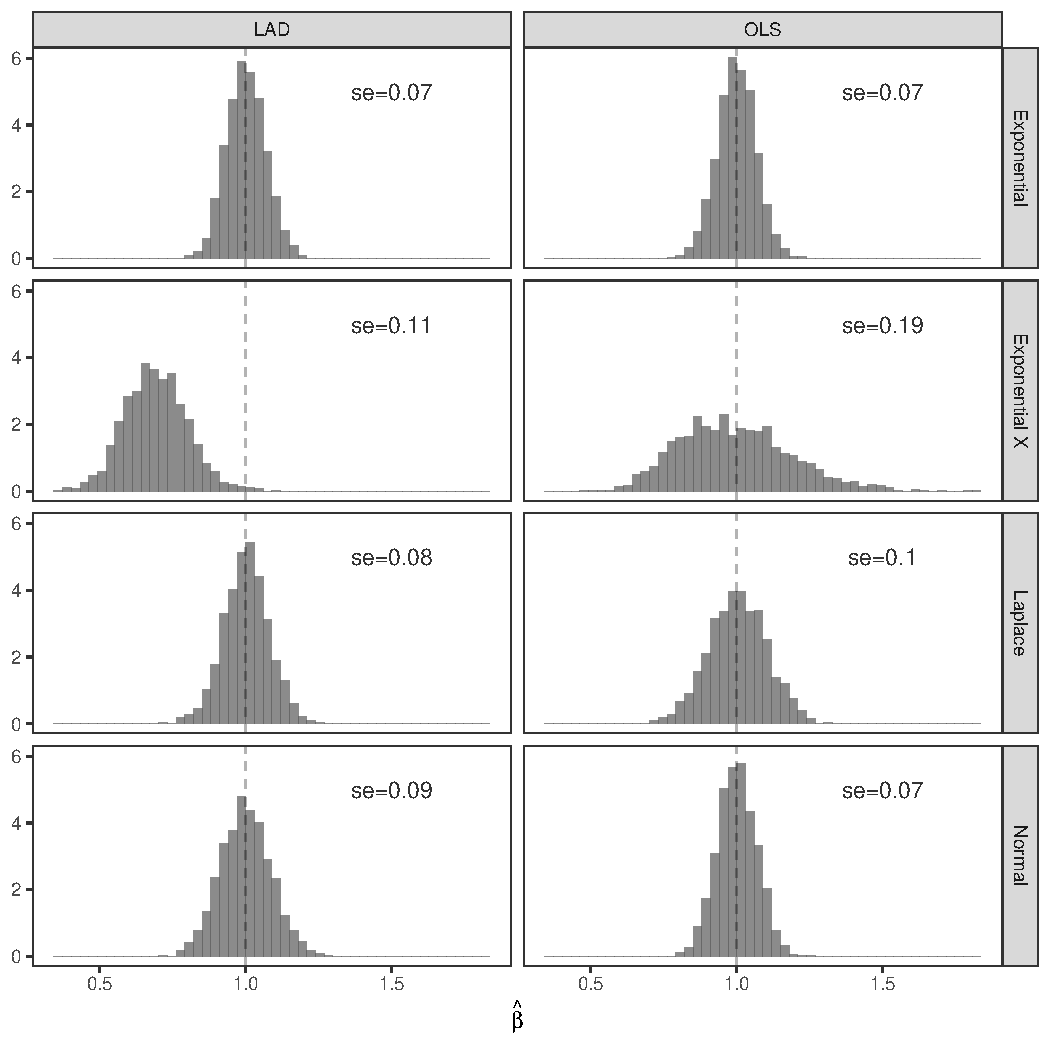
\includegraphics[width = \textwidth]{figures/quantile_regression_simu.pdf}
\caption{Regression quantiles}\label{fig::simu-regression-quantiles}
\end{figure}






\section{Application}

\subsection{Parents' and children's heights}



I revisit Galton's data introduced in Chapter \ref{chapter::ols-1d}. The following code gives the coefficients for quantiles $0.1$ to $0.9$. 

\begin{lstlisting}
> library("HistData")
> taus     = (1:9)/10
> qr.galton = rq(childHeight ~ midparentHeight, 
+                tau = taus,
+                data = GaltonFamilies)
> coef.galton = qr.galton$coef
\end{lstlisting} 



\begin{figure}[th]
\centering
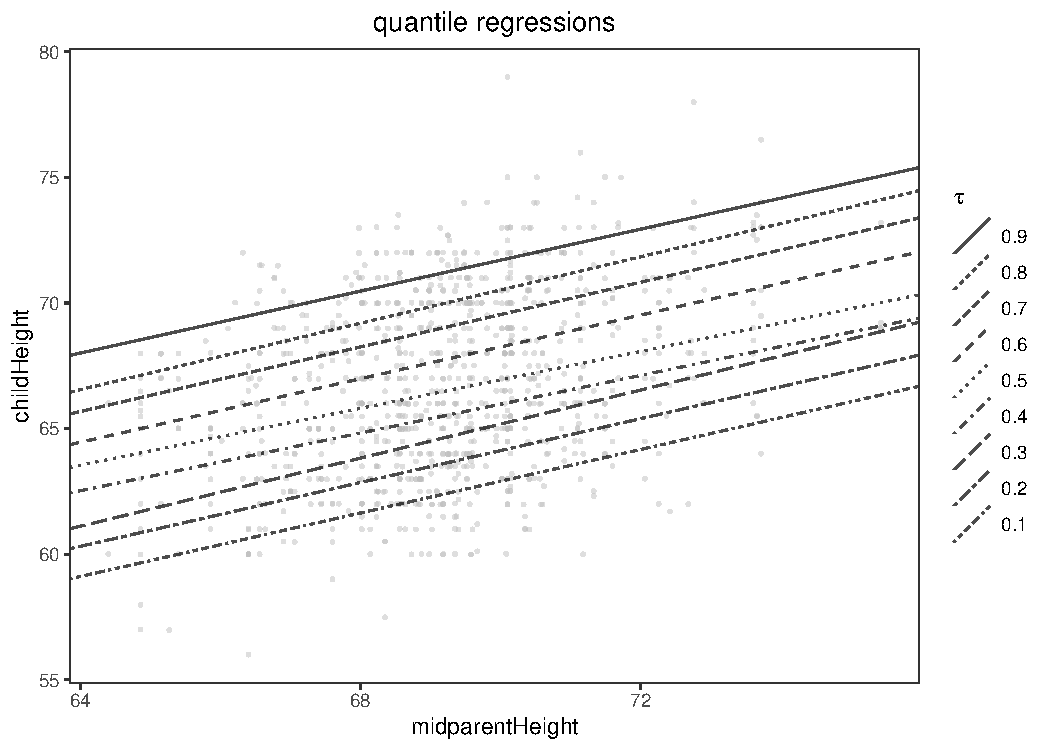
\includegraphics[width = 0.8 \textwidth]{figures/galton_qr.pdf}
\caption{Galton's data}\label{fig::galton-regression-quantiles}
\end{figure}


Figure \ref{fig::galton-regression-quantiles} shows the quantile regression lines, which are almost parallel with different intercepts. In Galton's data, $x$ and $y$ are very close to a bivariate Normal distribution. Theoretically, we can verify that with bivariate Normal $(x,y)$, the conditional quantile function $F^{-1}(\tau \mid x)$ is linear in $x$ with the same slope. See Problem \ref{hw22::qr-bivariate-Normal}. 





\subsection{U.S. wage structure}


\citet{angrist2006quantile} used quantile regression to study the U.S. wage structure. They used census data in 1980, 1990, and 2000 to fit quantile regressions on log weekly wage on education and other variables. The following code gives the coefficients for quantile regressions with $\tau$ equaling $0.1$ to $0.9$. I repeated the regressions with data from three years. Due to the large sample size, I use the $m$-of-$n$ bootstrap with $m=500$.


\begin{lstlisting}
> library(foreign)
> census80 = read.dta("census80.dta")
> census90 = read.dta("census90.dta")
> census00 = read.dta("census00.dta")
> f.reg = logwk ~ educ + exper + exper2 + black
> 
> m.boot   = 500       
> rq80     = rq(f.reg, data = census80, tau = taus)
> rqlist80 = summary(rq80, se = "boot", 
+                    bsmethod= "xy", mofn = m.boot)
> rq90     = rq(f.reg, data = census90, tau = taus)
> rqlist90 = summary(rq90, se = "boot", 
+                    bsmethod= "xy", mofn = m.boot)
> rq00     = rq(f.reg, data = census00, tau = taus)
> rqlist00 = summary(rq00, se = "boot", 
+                    bsmethod= "xy", mofn = m.boot)
\end{lstlisting}


Figure \ref{fig::angrist-regression-quantiles} shows the coefficient of \ri{educ} across years and across quantiles. In 1980, the coefficients are nearly constant across quantiles, showing no evidence of heterogeneity in the return of education. Compared with 1980, the return of education in 1990 increases across all quantiles, but it increases more at the upper quantiles. Compared with 1990, the return of education in 2000 decreases at the lower quantiles and increases at the upper quantiles, showing more dramatic heterogeneity across quantiles. 

 
\begin{figure}[th]
\centering
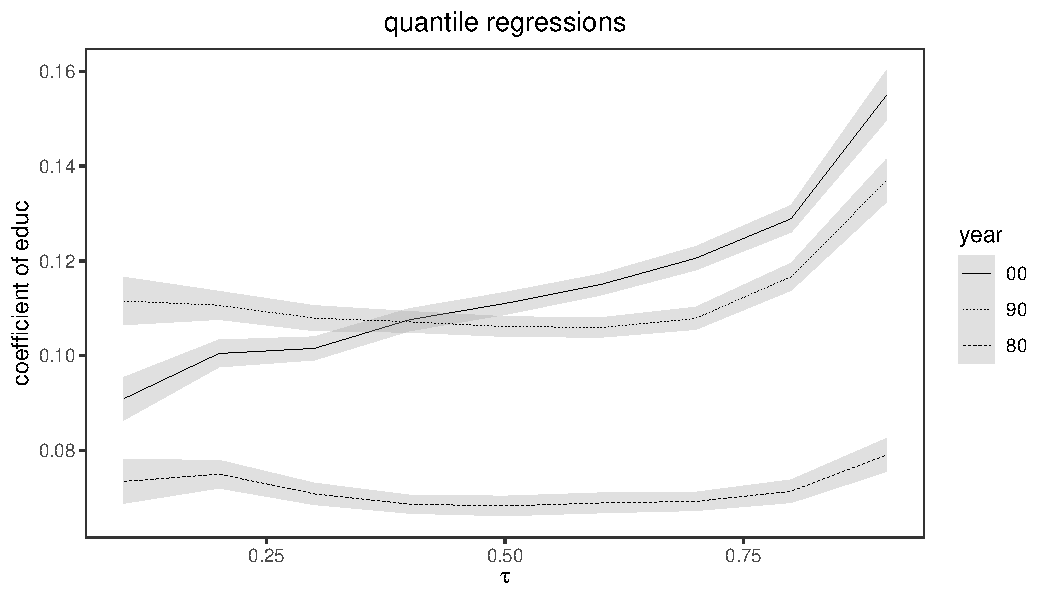
\includegraphics[width = \textwidth]{figures/angrist_qr.pdf}
\caption{\citet{angrist2006quantile}'s data}\label{fig::angrist-regression-quantiles}
\end{figure}



The original data used by \citet{angrist2006quantile} contain weights due to sampling. Ideally, we should use the weights in the quantile regression. Like \ri{lm}, the \ri{rq} function also allows for specifying \ri{weights}.

The \ri{R} code in this section is in \ri{code24.5.R}. 




\section{Extensions}


With clustered data, we must use the cluster-robust standard error which can be approximated by the clustered bootstrap with the \ri{rq} function. I use \citet{hagemann2017cluster}'s example below where the students are clustered in classrooms. See \ri{code24.6.R}. 

\begin{lstlisting}
> star = read.csv("star.csv")
> star.rq  = rq(pscore ~ small + regaide + black + 
+                 girl + poor + tblack + texp + 
+                 tmasters + factor(fe),
+               data = star)
> res      = summary(star.rq, se = "boot")$coef[2:9, ]
> res.clus = summary(star.rq, se = "boot", 
+                    cluster = star$classid)$coef[2:9, ]
> round(res, 3)
           Value Std. Error t value Pr(>|t|)
small      6.500      1.122   5.795    0.000
regaide    0.294      1.071   0.274    0.784
black    -10.334      1.657  -6.237    0.000
girl       5.073      0.878   5.777    0.000
poor     -14.344      1.024 -14.011    0.000
tblack    -0.197      1.751  -0.113    0.910
texp       0.413      0.098   4.231    0.000
tmasters  -0.530      1.068  -0.497    0.619
> round(res.clus, 3)
           Value Std. Error t value Pr(>|t|)
small      6.500      1.662   3.912    0.000
regaide    0.294      1.627   0.181    0.857
black    -10.334      1.849  -5.588    0.000
girl       5.073      0.819   6.195    0.000
poor     -14.344      1.152 -12.455    0.000
tblack    -0.197      3.113  -0.063    0.949
texp       0.413      0.168   2.465    0.014
tmasters  -0.530      1.444  -0.367    0.713
\end{lstlisting}




With high dimensional covariates, we can use regularized quantile regression. For instance, the \ri{rq} function can implement the lasso version with \ri{method = "lasso"} and a prespecified \ri{lambda}. It does not implement the ridge version. 






\section{Homework problems}
 
 

\paragraph{Quantile regression with a binary regressor}\label{hw22::qr-binaryx}

For $i=1,\ldots, n$, the first $1/3$ observations have $x_i=1$ and the last $2/3$ observations have $x_i=0$;
$y_i\mid x_i =1$ follows an Exponential$(1)$, and $y_i\mid x_i = 0 $ follows an Exponential$(2)$. Find
$$
(\hat{\alpha}, \hat{\beta})  = \arg\min_{(a,b)} \sumn \rho_{1/2}(y_i - a - b x_i).
$$
and the joint asymptotic distribution. 




\paragraph{Conditional quantile function in bivariate Normal}\label{hw22::qr-bivariate-Normal}

Show that if $(x,y)$ follows a bivariate Normal, the conditional quantile function of $y$ given $x$ is linear in $x$ with the same slope across all $\tau$. 

\paragraph{Quantile range and variance}\label{hw22::quantile-range-variance}

A symmetric random variable $y$ satisfies $y \sim -y$. 
Define the $1-\alpha$ quantile range of a symmetric random variable $y$ as the interval of its $\alpha/2$  and $1-\alpha/2$ quantiles. 
Given two symmetric random variables $y_1$ and $y_2$, show that if the $1-\alpha$ quantile range of $y_1$ is wider than that of $y_2$ for all $\alpha$, then $\var(y_1) \geq \var(y_2)$. Does the converse of the statement hold? If so, give a proof; if not, give a counterexample. 




\paragraph{Interquartile range and estimation}\label{hw22::interquartile-range}

The interquartile range of a random variable $y$ equals the difference between its 75\% and 25\% quantiles. 
Based on IID data $(y_i)_{i=1}^n$, write a function to estimate the interquartile range and the corresponding standard error using the bootstrap. Use simulated data to evaluate the finite sample properties of the point estimate (e.g., bias and variance) and the 95\% confidence interval (e.g. coverage rate and length). 


Find the asymptotic distribution of the estimator for the interquartile range. 

 

\paragraph{Joint asymptotic distribution of the sample median and the mean}
\label{hw22::joint-mean-median}

Assume that $y_1,\ldots, y_n \sim y$ are IID. Find the joint asymptotic distribution of the sample mean $\bar{y}$ and median $\hat{m}$.

Hint: The mean $\mu$ and median $m$ satisfy the estimating equation with 
$$
w(y, \mu, m) = \begin{pmatrix}
y - \mu \\
0.5 - 1(y - m \leq 0)
\end{pmatrix}. 
$$


\paragraph{Weighted quantile regression and application}\label{hw22::weighted-qr-application}

Many real data contain weights due to sampling. For example, in \citet{angrist2006quantile}'s data, \ri{perwt} is the sampling weight. Define the weighted quantile regression problem theoretically and re-analyze \citet{angrist2006quantile}'s data with weights. Note that similar to \ri{lm} and \ri{glm}, the quantile regression function \ri{rq}  also has a parameter \ri{weights}. 



 

